\documentclass{beamer}
\mode<presentation>{}

\usepackage{hyperref}
\usepackage{amsmath}
\usepackage{graphicx}
\usepackage{listings}
\usepackage{color}

\graphicspath{ {/Users/matthewdrury/Presentations/boosting-presentation-for-galvanize/plots/} }

\AtBeginSection[]{
  \begin{frame}
  \vfill
  \centering
  \begin{beamercolorbox}[sep=8pt,center,shadow=true,rounded=true]{title}
    \usebeamerfont{title}\insertsectionhead\par%
  \end{beamercolorbox}
  \vfill
  \end{frame}
}

\definecolor{mygreen}{rgb}{0,0.6,0}
\definecolor{mygray}{rgb}{0.5,0.5,0.5}
\definecolor{mymauve}{rgb}{0.58,0,0.82}

% Code formatting stuff.
\lstset{ %
  backgroundcolor=\color{white},   % choose the background color; you must add \usepackage{color} or \usepackage{xcolor}
  basicstyle=\scriptsize,          % the size of the fonts that are used for the code
  breakatwhitespace=false,         % sets if automatic breaks should only happen at whitespace
  breaklines=true,                 % sets automatic line breaking
  captionpos=b,                    % sets the caption-position to bottom
  commentstyle=\color{mygreen},    % comment style
  deletekeywords={...},            % if you want to delete keywords from the given language
  escapeinside={\%*}{*)},          % if you want to add LaTeX within your code
  extendedchars=true,              % lets you use non-ASCII characters; for 8-bits encodings only, does not work with UTF-8
  keepspaces=true,                 % keeps spaces in text, useful for keeping indentation of code (possibly needs columns=flexible)
  keywordstyle=\color{blue},       % keyword style
  language=Octave,                 % the language of the code
  otherkeywords={*,...},           % if you want to add more keywords to the set
  numbers=none,                    % where to put the line-numbers; possible values are (none, left, right)
  numbersep=5pt,                   % how far the line-numbers are from the code
  numberstyle=\tiny\color{mygray}, % the style that is used for the line-numbers
  showspaces=false,                % show spaces everywhere adding particular underscores; it overrides 'showstringspaces'
  showstringspaces=false,          % underline spaces within strings only
  showtabs=false,                  % show tabs within strings adding particular underscores
  stepnumber=2,                    % the step between two line-numbers. If it's 1, each line will be numbered
  stringstyle=\color{mymauve},     % string literal style
  tabsize=2,	                   % sets default tabsize to 2 spaces
  title=\lstname                   % show the filename of files included with \lstinputlisting; also try caption instead of title
}


\DeclareMathOperator*{\argmin}{arg\,min}
\DeclareMathOperator*{\bias}{bias}
\DeclareMathOperator*{\var}{var}
\DeclareMathOperator*{\tr}{tr}
\DeclareMathOperator*{\pd}{pd}
\DeclareMathOperator*{\goesto}{\rightarrow}
%\DeclareMathOperator*{\implies}{\Rightarrow}

\title{Probability and Statistics Short Course: Seattle}   
\author{Matthew Drury} 
\date{\today} 

\begin{document}


%
\begin{frame}
  \titlepage
\end{frame}
%

\frame{\frametitle{Table of contents}\tableofcontents} 

\section{Introduction} 

%
\frame{\Large

What is Probability?

What is Statistics?

What is the difference?

}%

%
\frame{\Large

\textbf{Probability} refers to the study of patterns in a random process.

When we solve problems in probability we assume that all basic features of the random process are \textbf{known}, and our goal is to discover other, deeper features.

}%

%
\frame{\Large

For example:

If I have a coin which is \textbf{known} to land head exactly half of the time, it is a problem in \textbf{probability} to determine how often the coin will never land on heads over ten consecutive flips.

}%

%
\frame{\Large

\textbf{Statistics} refers to the study of random process where some basic features of the random process are \textbf{unknown}, and our goal is to \textbf{infer from observations} basic, hidden features of the random process.

}%

\frame{\Large

For example:

It is a problem in \textbf{statistics} to determine, when presented with a coin which has landed tails ten consecutive times, whether one should continue to believe it fair.

}%

%
\frame{\Large

In this course:

\textbf{Day 1 (Tuesday):} Basics of Probability.

\textbf{Day 2 (Thursday):} Basics of Statistics.

}%
 % Introduction
\section{Counting (Combinatorics)}

%
\frame{ 
The basic problem solving skill you need to solve problems in probability is \textbf{counting} (no, really).
}%

%
\frame{

For example:

\begin{itemize}
\item How many ways are there to arrange four letters of the alphabet?
\item How many ways are there to arrange four \textit{different} letters of the alphabet.
\item How many ways are there to arrange 25 math books on a bookshelf.
\item How many five card hands are full houses.
\item How many five card hands have three of a kind.
\item How many five card hands have three of a kind and are not also full
houses.
\end{itemize}

}%

%
\frame{

\textbf{Basic Counting Principle}

\hfill

If a task can be accomplished as a series steps, then the number of outcomes of the task is the \textbf{product} of the number of outcomes of each individual step.

}%

%
\frame{

How many ways are there to arrange four letters of the alphabet?

\hfill

Think: How can we accomplish this task as a step by step process.

}%

%
\frame{

How many ways are there to arrange four letters of the alphabet?

\hfill

Think: How can we accomplish this task as a step by step process.

\hfill

Pick the first letter, write it down.

$\Rightarrow$ Pick the second letter, write it down.

$\Rightarrow$ Pick the third letter, write it down.

$\Rightarrow$ Pick the fourth letter, write it down.

}%

%
\frame{

$$ 26 \times 26 \times 26 \times 26 = 456976 $$

}%

%
\frame{

How would this change if we could \textbf{not} re-use a letter?

}%

%
\frame{

The previous example is a common situation:  we are pulling from a pool of objects, and we \textbf{cannot} re-use an object once selected.

\hfill

This is called \textbf{selection without replacement}.

}%

\frame{

The number of \textbf{ordered} selections \textbf{of k objects} without replacement \textbf{from a population for k objects} is called the \textbf{number of permutations of k objects taken from n}.

$$ P(n, k) = \underbrace{n \times (n-1) \times (n-2) \times \ldots \times (n - k + 1)}_{\text{k total factors}} $$

}%


%
\frame{

You have 25 math and stats books on a bookshelf.  How many ways are there to arrange these books in any order?

}%

%
\frame{

$$ 25 \times 24 \times 23 \times \ldots \times 2 \times 1 = 15511210043330985984000000 $$

}%

%
\frame{

What if we have a procedure in which the order of choices does not matter?

\hfill

How many 5 card hands are possible when drawing from a standard 52 card deck?

\hfill

Notice that the \textbf{order in which we draw cards is not important here}.

}%

%
\frame{

\textbf{Think:} To choose an \text{ordered} list of five cards I can \text{first} chose the five cards I want to use \text{and then} choose a way to order them.

\begin{align*}
\text{\# of} & \text{ ordered hands} \\
&= \text{\# of unordered hands} \times \text{\# of ways to order five cards}
\end{align*}

}%

%
\frame{

$$ 52 \times 51 \times 50 \times 49 \times 48 = \text{\# of unordered hands} \times 5 \times 4 \times 3 \times 2 \times 1 $$

}%

%
\frame{

$$ \text{\# of unordered hands} = \frac{52 \times 51 \times 50 \times 49 \times 48}{5 \times 4 \times 3 \times 2 \times 1} $$

}

%
\frame{

The number of \text{unordered} selections \textbf{of k objects} without replacement \textbf{from a population for k objects} is called the \textbf{number of combinations of k objects taken from n}.

$$ C(n, k) = \frac{P(n, k)}{P(k, k)} $$

Another common notation:

$$ {{n}\choose{k}} = \frac{P(n, k)}{P(k, k)} $$ 

}%

%
\frame{

\begin{align*}
\text{\# of} & \text{ unordered collections something} \\
&= \frac{ \text{\# of ordered sequences of the thing}} {\text{\# of ways to
order a single sequence}}
\end{align*}

}%

%
\frame{

A \textbf{full house} is a hand of five cards that has a \textbf{pair} of the same value, and a \textbf{three of a kind} of the same value.  How many hands of five cards are full houses?

}

%
\frame{

A \textbf{full house} is a hand of five cards that has a \textbf{pair} of the same value, and a \textbf{three of a kind} of the same value.  How many hands of five cards are full houses?

\hfill

Choose a value for the pair

$\Rightarrow$ Choose two cards of that value

$\Rightarrow$ Chose a value for the three of a kind

$\Rightarrow$ Choose three cards of that value

}%

%
\frame{

A \textbf{full house} is a hand of five cards that has a \textbf{pair} of the same value, and a \textbf{three of a kind} of the same value.  How many hands of five cards are full houses?

\hfill

Choose a value for the pair

$\Rightarrow$ Choose two cards of that value

$\Rightarrow$ Chose a value for the three of a kind

$\Rightarrow$ Choose three cards of that value

$$ 13 \times C(4, 2) \times 12 \times C(4, 3) = 13 \times 6 \times 12 \times 4 = 3744 $$

}%

%
\frame{

How many hands are there that contain a three-of-kind that are not full houses?

}%
 % Counting principles
\section{Probability Basics}

%
\begin{frame}

An \textbf{outcome} is a single thing that can happen.

\hfill

An \textbf{event} is a collection of things that can happen, usually given by a
short description.

\end{frame}
%

%
\begin{frame}

For example:

\hfill

When thinking about poker hands, an \textbf{outcome} is a single hand (any
unordered collection of five cards).

\hfill

The collection of all full-houses, three of a kinds, etc are \textbf{events}.

\end{frame}


%
\begin{frame}

The \textbf{probability} of an event is:

$$ P(\text{event}) = \frac{\text{\# of ways event can happen}}{\text{total \# of
things that can happen}} $$

So to compute basic probabilities, we use our knowledge from counting.

\end{frame}
%

%
\begin{frame}

$$ P(\text{full-house}) = \frac{\text{\# of full houses}}{\text{total \# of
hands}} $$

\end{frame}
%

%
\begin{frame}

$$ \text{\# of full houses} = 13 \times 6 \times 12 \times 4 = 3744 $$

$$ \text{total \# of hands} = {{52}\choose{5}} = 2598960 $$

\end{frame}
%

%
\begin{frame}

$$ P(\text{full-house}) = \frac{3744}{2598960} = 0.0014 $$

\end{frame}
%

%
\begin{frame}

What is the probability of drawing a hand containing a three of a kind \textbf{that is
not a full house or four of a kind}?


\end{frame}
 % Probability from counting
\section{Conditional Probability}

%
\begin{frame}

Suppose we know that one event $C$ has already happened or will happen (the
condition), and we want to know the probability of different event $B$.

\hfill

Then the \textbf{conditional probability of $A$ given $B$} is defined by

$$ P(A \mid B) = \frac{\text{\# of ways A and B \textbf{both} happen}}{\text{\#
of ways B can happen}} $$

\end{frame}
%

%
\begin{frame}

What is the conditional probability that you draw a hand containing a three of a
kind, given that you draw a hand containing a pair?

\begin{align*}
P(\text{Drawing a} & \text{ three of a kind} \mid \text{Drawing a pair}) = \\ 
&= \frac{\text{\# of ways of drawing a three of a kind}}{\text{\# of ways of
drawing a pair}}
\end{align*}

\textbf{Important}: Any hand containing a three of a kind \textbf{automatically}
contains a pair!

\end{frame}
%

%
\begin{frame}

$$ \text{\# of ways of drawing a three of a kind} = 13 \times {{4}\choose{3}}
\times {{49}\choose{2}} = 61152 $$

$$ \text{\# of ways of drawing a pair} = 13 \times {{4}\choose{2}}
\times {{50}\choose{3}} = 1528800 $$

\end{frame}
%

%
\begin{frame}

\begin{align*}
P(\text{Drawing a} & \text{ three of a kind} \mid \text{Drawing a pair}) = \\ 
&= \frac{61152}{1528800} \\
&= 0.04
\end{align*}

\end{frame}
%

%
\begin{frame}

There is another way to look at conditional probabilities

\begin{align*}
P(A & \mid B) & \\
%
&= \frac{\text{\# of ways A and B \textbf{both} happen}}{\text{\#
of ways B can happen}} \\[0.5ex]
%
&= \frac{\frac{\text{\# of ways A and B \textbf{both} happen}}{\text{Total \# of
things that can happen}}}{\frac{\text{\# of ways B can happen}}{\text{Total \# of
things that can happen}}} \\[0.5ex]
%
&= \frac{P(A \text{ and } B)}{P(B)}
\end{align*}

\end{frame}
%

%
\begin{frame}

So we could have instead computed:

\begin{align*}
P(\text{Drawing a} & \text{ three of a kind} \mid \text{Drawing a pair}) = \\
%
&= \frac{P(\text{Drawing a three of a kind})}{P(\text{Drawing a pair})} \\
%
&= \frac{\frac{61152}{2598960}}{\frac{1528800}{2598960}} \\
%
&= \frac{0.024}{0.588} \\
%
&= 0.04
\end{align*}

\end{frame}
%

%
\begin{frame}

What is the conditional probability that you draw a full house, given that you know you
have at least a three of a kind

\begin{align*}
P(\text{Drawing a} & \text{ full house} \mid \text{Drawing a three of a kind}) = \\
%
&= \frac{\text{\# of ways of drawing a full house}}{\text{\# of ways of drawing
a three of a kind}} \\
%
&= \frac{ 13 \times {{4}\choose{3}} \times 12 \times {{4}\choose{2}} } {13
\times {{4}\choose{3}} \times {{50}\choose{2}}} \\
%
&= \frac{3744}{63700} \\
%
&= 0.059
\end{align*}

\end{frame}
%

%
\begin{frame}
What is the conditional probability that you draw a full house, given that you
have drawn a four of a kind.

What is the conditional probability that you draw a four of a kind, given that
you know you already have a pair?
\end{frame}

\begin{frame}

Two events $A$ and $B$ are called \textbf{independent} when

$$ P(A \mid B) = P(A) $$

This means that \textbf{knowledge that B has or will occur does not change our
knowledge about whether A will occur}.

\end{frame}
%

%
\begin{frame}

Remember that the definition of conditional probability is

$$ P(A \mid B) = \frac{P(A \text{ and } B)}{P(B)} $$

Combining this with our definition of independence (so, below, $A$ and $B$ are
independent

$$ P(A) = P(A \mid B) = \frac{P(A \text{ and } B)}{P(B)} $$

Or, rearranging things

$$ P(A \text{ and } B) = P(A) P(B) $$

This equation is sometimes used as the \textbf{definition} of independence,
though I think it is less convincing.

\end{frame}
%

%
\begin{frame}

Common applications of independence generally go like this:

\begin{itemize}
\item We deduce from context that some event bears no influence on another.
\item We conclude that the two events are independent.
\item We use either of the two equations defining independence to fo
calculations.
\end{itemize}

\end{frame}
%

%
\begin{frame}

You roll a six sided die six times, what is the probability that you roll
\textbf{all
the possible numbers, in decreasing order}?

\end{frame}
%

%
\begin{frame}

Let's call the values of the rolls $R_1, R_2, R_3, R_4, R_5$ and $R_6$.  Then we
are looking for

$$P(R_1 = 6 \text{ and } R_2 = 5 \text{ and } R_3 = 4\text{ and } R_4 = 3 \text{
and } R_5 = 2 \text{ and } R_6 = 1)$$

Since each individual roll of the die does not influence the others, all size
rolls are independent.  This means we can break up and multiply

$$ P(R_1 = 6) \times P(R_2 = 5) \times P(R_3 = 4) \times P(R_4 = 3) \times P(R_5
= 2) \times P(R_6 = 1) $$

\end{frame}
%

%
\begin{frame}
Since each individual roll of the die has \textbf{six possible outcomes} and
\textbf{only one of them is the number we are looking for} we get

$$ P(\cdots) = \frac{1}{6} \times \frac{1}{6} \times \frac{1}{6} \times
\frac{1}{6} \times \frac{1}{6} \times \frac{1}{6} = \frac{1}{46656} $$
\end{frame}
%

%
\begin{frame}
Suppose you have a bucket with 5 red and 5 yellow balls in it, which you draw in
sequence, without replacement.  Are the events "You draw a red ball first" and 
"You draw a yellow ball second" independent?

Suppose that it rains with probability $80 \%$ each day in seattle, and a winter
month has four work weeks.  What is the probability that there is a work week in
which it rains \textbf{every day}?  What assumptions do you have to make to
solve this problem?  Are they reasonable?
\end{frame}

\section{Bayes' Formula}

%
\begin{frame}
Remember our definition of conditional probability:

\begin{align*}
P(A \text{ and } B) &= P(A \mid B) P(B) \\
P(B \text{ and } A) &= P(B \mid A) P(A) \\
\end{align*}

Setting these equal to one another leads us to \textbf{Bayes' Formula}

$$ P(A \mid B) = \frac{ P(B \mid A) P(A) }{ P(B) } $$

\end{frame}
%

%
\begin{frame}

This is probably the most important simple formula in both probability and
statistics

$$ P(A \mid B) = \frac{ P(B \mid A) P(A) }{ P(B) } $$

\end{frame}
%

%
\begin{frame}

Let's study a classic thought experiment: the disease screening problem.

Suppose we have developed a test for a certain disease:
\begin{itemize}
\item Only 1 \% of people have the disease.
\item If a person has the disease, the test will be positive 99.9 \% of the
time.
\item If a person does not have the disease, the test will be negative 98 \% of
the time.
\end{itemize}

You get tested for the disease, and the test is positive.  \textbf{What is the
probability that you actually have the disease}?

\end{frame}
%

%
\begin{frame}
We are after the following conditional probability

$$ P(\text{Have Disease} \mid \text{Test is Positive)} $$

And we \textbf{know}

$$ P(\text{Have Disease}) = 0.01 $$
$$ P(\text{Test is Positive} \mid \text{Have Disease}) = 0.999 $$
$$ P(\text{Test is Positive} \mid \text{Do Not Have Disease}) = 0.02 $$
\end{frame}
%

%
\begin{frame}
Bayes theorem says:

\begin{align*}
P(\text{Have Disease}  & \mid \text{Test is Positive)} = \\
%
& = \frac{  P(\text{Test is
Positive} \mid \text{Have Disease}) P(\text{Have Disease}) } { P(\text{Test is
Positive}) }
\end{align*}

We know all the things appearing in this formula except $ P(\text{Test is
Positive}) $.

\end{frame}
%

%
\begin{frame}

We can calculate the last piece by breaking things down

\begin{align*}
P(\text{Test} & \text{ is Positive}) \\
%
&= P(\text{Test is Positive and Have Disease}) \\
%
& \quad + P(\text{Test is Positive and Don't Have Disease}) \\
\end{align*}

\end{frame}
%

%
\begin{frame}

\begin{align*}
P(\text{Test} & \text{ is Positive and Have Disease}) \\
%
=& P(\text{Test is Positive} \mid \text{Have Disease}) P(\text{Have Disease}) \\
=& 0.999 \times 0.01 \\
\end{align*}

\end{frame}
%

%
\begin{frame}

\begin{align*}
P(\text{Test} & \text{ is Positive and Don't Have Disease}) \\
%
=& P(\text{Test is Positive} \mid \text{Don't Have Disease}) P(\text{Don't Have Disease}) \\
=& 0.02 \times 0.99 \\
\end{align*}

\end{frame}


\begin{frame}

We have all the pieces, so let's put them together

\begin{align*}
P(\text{Have Disease}  & \mid \text{Test is Positive}) = \\
%
&= \frac{  P(\text{Test is
Positive} \mid \text{Have Disease}) P(\text{Have Disease}) } { P(\text{Test is
Positive}) } \\
%
&= \frac{ 0.999 \times 0.01 } {  0.999 \times 0.01 +  0.02 \times 0.99 } \\
%
&= 0.34
\end{align*}

The probability we have the disease is called only 34 \%, \textbf{even after we
have received a positive test}.

\end{frame}
%

%
\begin{frame}

This kind of result is unintuitive to almost all humans, a mental bias called the
\textbf{base rate fallacy}.

Pretty much \textbf{everyone's} intuition says that it should be much more
likely that the person does have the disease after a test comes back positive.
Pretty much \textbf{everyone} undervalues the prior information that

$$ P(\text{Have Disease}) = 0.01 $$

\textbf{I takes a lot of evidence to take an unlikely situation and make it
likely.}

\end{frame}
%

%
\begin{frame}
There is some terminology that is often used to understand these relationships:

\begin{itemize}
\item $P(\text{Have Disease})$ is called the \textbf{prior probability}.  It is
what we know \textbf{before collecting evidence/data}.
\item $P(\text{Test is Positive} \mid \text{Have Disease})$ is called the
\textbf{likelihood}.  It is the \textbf{strength of the evidence/data we collected}.
\item $P(\text{Have Disease } \mid \text{Test is Positive})$ is called the
\textbf{posterior}.  It is what we know, \textbf{after collecting evidence/data}.
\end{itemize}

These ideas form the basis of \textbf{Bayesian statistics}.

\end{frame}
%

\section{Random Variables}

\begin{frame}
A random variable $X$ is an object that can be used to generate numbers, in a way that valid probabilistic statements about the generated numbers can be made. 

\hfill

For example:
$$ P(X > 0) = 0.25 $$
$$ P(-1 < X < 1) = 0.25 $$
$$ P(X < -1) = 0.02 $$
$$ P(X > 1 \mid X > 0) = 0.5 $$

Are all probabilistic statements about an unknown random variable $X$.
\end{frame}
%

%
\begin{frame}
Random variables can be used to model real life events or measurements when
there is some variation in their outcomes that we cannot account for

\begin{itemize}
\item The number of heads seen in ten flips of a quarter.
\item The number of heads seen in ten flips of a dime.
\item The number of Buses that arrive late to a stop in Seattle in a single
day.
\item The number of times my cat asks for food between 5 and 6 pm (when she is
always fed) in a given day.
\item The temperature on a mid-summers day in Seattle.
\item The rainfall in a mid-winters day in Seattle.
\end{itemize}

\end{frame}
%

%
\begin{frame}
We naturally have a feeling that there is something \textbf{the same} about
these two situations

\begin{itemize}
\item The number of heads seen in ten flips of a quarter.
\item The number of heads seen in ten flips of a dime.
\end{itemize}

What is it?
\end{frame}
%

%
\begin{frame}

We expect that the probabilities

$$ P(\text{We get 5 heads in 10 flips of a quarter}) $$
$$ P(\text{We get 5 heads in 10 flips of a dime}) $$

are \textbf{equal}.

\hfill

So are

$$ P(\text{We get 2 heads in 10 flips of a quarter}) $$
$$ P(\text{We get 2 heads in 10 flips of a dime}) $$

and so on...
\end{frame}
%

%
\begin{frame}
The \textbf{sameness} that we sense between

\begin{itemize}
\item The number of heads seen in ten flips of a quarter.
\item The number of heads seen in ten flips of a dime.
\end{itemize}

is that the probabilities of all events like

$$ P(\text{We get } N \text{ heads in 10 flips of a quarter}) $$
$$ P(\text{We get } N \text{ heads in 10 flips of a dime}) $$

\textbf{are all equal}.
\end{frame}
%

%
\begin{frame}
We summarize this by saying that the random variables


\begin{itemize}
\item The number of heads seen in ten flips of a quarter.
\item The number of heads seen in ten flips of a dime.
\end{itemize}

\textbf{have the same distribution}.

\hfill

The \textbf{distribution} of a random variable is the pattern of all
probabilities we assign to all outcomes of the random variable.
\end{frame}

%
\begin{frame}
So two random variables have the same distribution if \textbf{they assign the
same probabilities to all of the possible outcomes}.

\hfill

In this case, we use the shorthand \textbf{equally distributed}.
\end{frame}
%

\section{Common Distributions}

\begin{frame}
Some distributions are so common, they have been named and entered our shared
statistical conciousness.
\end{frame}
%

%
\begin{frame}{Bernoulli Distribution}
A single coin flip is an example of a \text{Bernoulli Distributed} random
variable.

The \textbf{Bernoulli distribution} describes any random event with only two possible
outcomes.
\end{frame}
%

%
\begin{frame}

We can draw a picture of a distribution by letting the hight of bars represent
the probabilities of certain outcomes occuring:

  \begin{figure}
    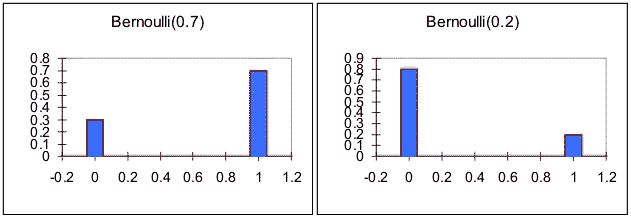
\includegraphics[scale=0.40]{bernoulli}
  \end{figure}

This picture is called the \textbf{probability mass function} of the
distribution.
\end{frame}
%

%
\begin{frame}

  \begin{figure}
    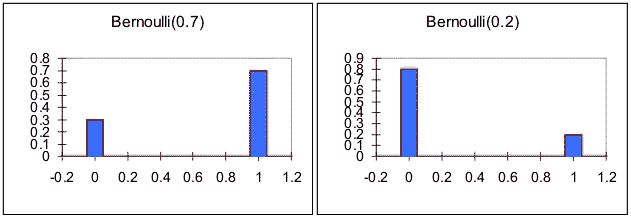
\includegraphics[scale=0.40]{bernoulli}
  \end{figure}

Notice how the first picture represents the occurance of a \textbf{common event}
and the second a \text{rare event}.

\hfill

Changing the probability that the event occurs changes the shape of the
probability mass function. This is called \textbf{varying a parameter}.

\end{frame}
%

%
\begin{frame}
Draw pictures of the probability mass functions of the following Bernoulli
distributions:

\begin{itemize}
\item Flipping a fair coin.
\item Rolling a six on a six sided die.
\item Rolling a twenty on a twenty sided die.
\item Rolling greater than a ten on a twenty sided die.
\end{itemize}

Are any of these equally distributed?
\end{frame}
%

%
\begin{frame}{Binomial Distribution}
The two familiar random variables

\begin{itemize}
\item The number of heads seen in ten flips of a quarter.
\item The number of heads seen in ten flips of a dime.
\end{itemize}

Have a \textbf{binomial distribution}.
\end{frame}
%

%
\begin{frame}

\begin{align*}
P(\text{We get} & \text{ 2 heads in 10 flips of a quarter}) \\
%
&= {{10}\choose{2}} \times \left(\frac{1}{2} \right)^{10} \\
%
&= 0.044
\end{align*}

\end{frame}
%

%
\begin{frame}

The \textbf{binomial distribution} describes the number of events that happen in
a fixed number of \textbf{attempts} when the events \textbf{individually happen
with the same probability}.

\end{frame}
%

%
\begin{frame}
When we are flipping a fair coin, the heads happen with probability $\frac{1}{2}$, and

\begin{align*}
P(\text{We get} & \text{ k heads in n flips of a quarter}) \\
%
&= {{n}\choose{k}} \times \left(\frac{1}{2} \right)^n
\end{align*}

\end{frame}
%

%
\begin{frame}
If the coin in \textbf{unfair}, so that the probability of an individual head is
$p$, then

\begin{align*}
P(\text{We get} & \text{ k heads in n flips of a quarter}) \\
%
&= {{n}\choose{k}} \times p^k \times (1 - p)^{n - k}
\end{align*}

\end{frame}
%

%
\begin{frame}
The binomial distribution has \textbf{two parameters}:

\begin{itemize}
\item The number of attempts, usually called $n$.
\item The probability the event occurs in a single attempt, usually called $p$.
\end{itemize}

\end{frame}
%

%
\begin{frame}
Changing either $n$ or $p$ changes the shape of the binomial probability mass
function.

  \begin{figure}
    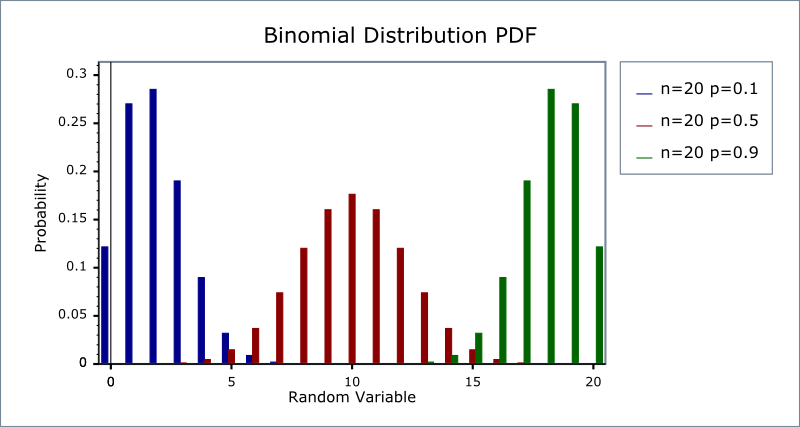
\includegraphics[scale=0.50]{binomial-pdf-changing-p}
  \end{figure}

\end{frame}
%

%
\begin{frame}

  \begin{figure}
    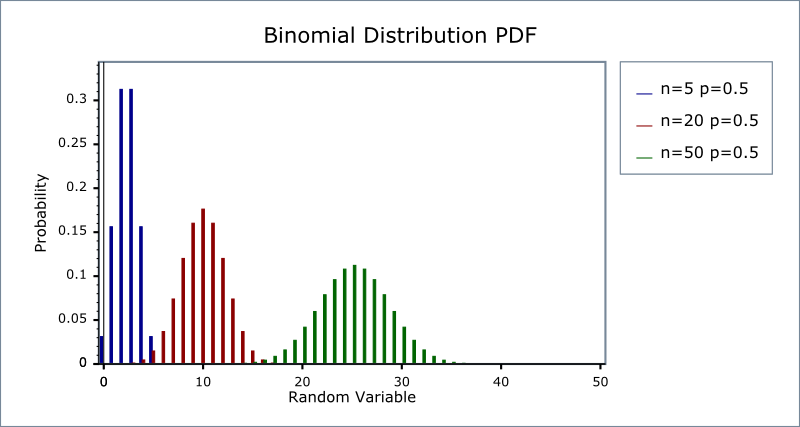
\includegraphics[scale=0.5]{binomial-pdf-changing-n}
  \end{figure}

\end{frame}
%

%
\begin{frame}

A \text{critical hit} is a roll of 20 on a 20 sided die.  In a session of
Dungeons and Dragons, you roll the die 20 times.  What is the probability that
you roll \textbf{at least two} critical hits.

\hfill

A \text{saving throw} is a roll of at least 15 on a 20 sided die.  In a sesson
of Dungeons and Dragons you roll the die to attept a saving throw 10 times.
What is the probability you \text{fail} all of your saving throws?

\end{frame}
%

%
\begin{frame}

In the two examples

\begin{itemize}
\item The number of buses that arrive late to a stop in Seattle in a single
day.
\item The number of times my cat asks for food between 5 and 6 pm (when she is
always fed) in a given day.
\end{itemize}

We see a similarity: they are both about the number of times an event happens
\textbf{in a given span of time (or space)}.
\end{frame}
%

%
\begin{frame}
If we assume that the buses arrive at a fixed rate (but possibly unknown), and
the cat meows at a fixed rate, then these are both examples of the
\textbf{Poisson Distribution}.

$$ P(\text{Cat meows k times in one hour}) = e^{-\lambda} \frac{\lambda^k}{k!}
$$

The $\lambda$ above is the \textbf{rate the event occurs}.
\end{frame}
%

%
\begin{frame}
Suppose we observe the cat meow 5 times in ten minutes.  What is the probability
that the cat will not meow at all in the next five minutes?
\end{frame}
%

%
\begin{frame}
The rate the cat meows is:

$$ \lambda = \frac{5 \text{ meows}}{10 \text{ minuets}} = 5 \frac{ \text{
meows}}{\text{ 10 minuets}} $$

So using the Poisson equation

$$ P(\text{Cat meows zero times in ten minuets}) = e^{-5} \frac{5^0}{0!} = 0.007
$$
\end{frame}
%

%
\begin{frame}
What is the probability the cat meows zero times in the next hour?

$$ 
\lambda = \frac{5 \text{ meows}}{10 \text{ minuets}} = 30 \frac{ \text{
meows}}{\text{ 60 minuets}} = 30 \frac{ \text{
meows}}{\text{ hour}}
$$

$$ P(\text{Cat meows zero times in the next hour}) = e^{-30} \frac{5^0}{0!} =
9.3 \times 10^{-14}
$$

Its basically impossible.
\end{frame}
%

%
\begin{frame}
The $n$ in a binomial distribution and the $\lambda$ in Poisson distribution are
called \textbf{parameters}.

The general strategy for solving problems like is:

\begin{itemize}
\item Use the information in the statement of the problem to determine a likely
distribution for the quantity of interest.
\item Use the information in the problem to determine the values to use for the
parameters of this distribution.
\item Use the probability function of the distribution to compute the needed
probability.
\end{itemize}

\end{frame}
%

%
\begin{frame}

Other distributions to know:

\begin{itemize}
\item Normal Distribution.  \textbf{Parameters:} The mean $\mu$, and the
standard deviation $\sigma$.
\item Uniform Distribution. \textbf{Parameters:} The minimum $a$ and the maximum
$b$.
\item Exponential Distribution. \textbf{Parameters:} The rate $\alpha$.
\end{itemize}

\end{frame}



\end{document}
